% !TeX program = pdfLaTeX
\documentclass[smallextended]{svjour3}       % onecolumn (second format)
%\documentclass[twocolumn]{svjour3}          % twocolumn
%
\smartqed  % flush right qed marks, e.g. at end of proof
%
\usepackage{amsmath}
\usepackage{graphicx}
\usepackage[utf8]{inputenc}

\usepackage[hyphens]{url} % not crucial - just used below for the URL
\usepackage{hyperref}
\providecommand{\tightlist}{%
  \setlength{\itemsep}{0pt}\setlength{\parskip}{0pt}}

%
% \usepackage{mathptmx}      % use Times fonts if available on your TeX system
%
% insert here the call for the packages your document requires
%\usepackage{latexsym}
% etc.
%
% please place your own definitions here and don't use \def but
% \newcommand{}{}
%
% Insert the name of "your journal" with
% \journalname{myjournal}
%

%% load any required packages here



\usepackage{booktabs}
\usepackage{longtable}
\usepackage{array}
\usepackage{multirow}
\usepackage{wrapfig}
\usepackage{float}
\usepackage{colortbl}
\usepackage{pdflscape}
\usepackage{tabu}
\usepackage{threeparttable}
\usepackage{threeparttablex}
\usepackage[normalem]{ulem}
\usepackage{makecell}
\usepackage{xcolor}

\begin{document}

\title{Do moral communities have a spatial dimension? A spatial exploratory
analysis of places of worship and violent crime in the city of Recife,
Brazil \thanks{Grants or other notes about the article that should go on the front page
should be placed here. General acknowledgments should be placed at the
end of the article.} }


    \titlerunning{Moral communities and crime}

\author{  Äüthör 1 \and  Âuthóř 2 \and  }


\institute{
        Äüthör 1 \at
     Department of YYY, University of XXX \\
     \email{\href{mailto:abc@def}{\nolinkurl{abc@def}}}  %  \\
%             \emph{Present address:} of F. Author  %  if needed
    \and
        Âuthóř 2 \at
     Department of ZZZ, University of WWW \\
     \email{\href{mailto:djf@wef}{\nolinkurl{djf@wef}}}  %  \\
%             \emph{Present address:} of F. Author  %  if needed
    \and
    }

\date{Received: date / Accepted: date}
% The correct dates will be entered by the editor


\maketitle

\begin{abstract}
A wealth of research exists to suggest that environmental attributes can
facilitate or deter criminal activities, as for instance the presence of
alcohol outlets or the design of defensible spaces. In this article we
present an exploratory spatial analysis of the relationship between
violent crime and places of worship in Recife, Brazil. This analysis
aims to explore whether there is a spatial dimension to ``moral
communities'' around places of worship. Use of a cluster detection
methodology, the results suggest the presence of a strong geographical
association between churches and crime. The evidence obtained for the
year 2010 indicates a process of clustering of homicide events in the
vicinity of places of worship. In addition, it was also possible to
verify a pattern of concentration between evangelical churches and
violent crimes.
\\
\keywords{
        Moral communities \and
        Crime \and
        Places of worship \and
        Point pattern analysis \and
        Intensity \and
    }


\end{abstract}


\def\spacingset#1{\renewcommand{\baselinestretch}%
{#1}\small\normalsize} \spacingset{1}


\hypertarget{intro}{%
\section{Introduction}\label{intro}}

Violent crime is a widespread phenomenon with negative impacts on many
spheres of life and society. Although the rate of homicides worldwide
has grown at a slower rate than the population, the number of people
killed in homicides still increased from 362,000 in 1990 to 464,000 in
2017 (United Nations Office on Drugs and Crime 2019a). Variations in
violent crime also tend to be extremely uneven. The Americas, with a
population of approximately 793.8 million people in 2019 (or about
10.3\% of the world population), accounted for approximately 173,000
homicides in 2017, or approximately 37.3\% of all homicides in the
world. Within the Americas, Brazil (along with Venezuela, Colombia, and
Mexico) is one of the largest countries in the region with high homicide
rates. The relevance of variations in the prevalence of violent crime is
in fact recognized by the United Nations Office on Drug and Crime
(2019a) as being key to achieving policy goals:

\begin{quote}
\begin{quote}
High levels of homicidal violence are concentrated in geographic and
demographic ``pockets'', so achieving target 16.1 of the Sustainable
Development Goals requires interventions within the specific regions,
countries, communities and population groups that are most at risk
(p.~35)
\end{quote}
\end{quote}

The endemic malady of violent crime represents in fact an important
factor that threatens to derail sustainable development goals. Violent
crime, furthermore, tends to be more accute in those regions most in
need of development. On the one hand, violent crime represents an
economic and social drag (Becker and Kassouf 2017) that affects people's
well-being, either through the loss of human life, mental health,
limitations in the right to public spaces (Doran and Burgess 2011), or
through disturbances in schooling and academic achievement (United
Nations Office on Drugs and Crime 2019b). In turn, these negative
effects combine to create the unfortunate conditions that exacerbate
criminal behavior, thus creating a vicious cycle of economic
disadvantage and crime (United Nations Office on Drugs and Crime 2019b).
Added to this scenario, social control institutions in Brazil, which in
practice should inhibit criminal practice, have deep deficiencies that
end up reducing the deterrent power of the criminal justice system.
Among these serious problems are the inefficiency of the police, the
lack of national legislation, the glacial pace of judicial processes.
and the weak situation of the prison system in the country (Menezes et
al. 2013). It is not surprising, given the above, that researchers have
joined calls for more research to increase our understanding of the
patterns of violent crime in Low and Middle Income Countries (LMIC;
Murray, Cerqueira, and Kahn 2013).

In order to counteract any criminological factors, it is important to
identify empirical regularities. Criminological factors include concrete
elements, such as the presence of arms or drugs, as well as
environmental factors, such as the built environment, in addition to
figurative factors, which include the moral costs of deviant behavior as
well as family supervision. Accordingly, a number of studies have
investigated various aspects of the environment and neighborhood design
(e.g., Foster, Giles-Corti, and Knuiman 2010; He, Páez, and Liu 2017;
Loukaitou-Sideris et al. 2001), whereas other studies have focused on
exposure to environmental attributes that signal weakened norms, such as
liquor and tobacco outlets associated with geographical hotspots of
crime (Brower and Carroll 2007; Deryol et al. 2016; Lipton et al. 2008;
Quick, Law, and Luan 2017). Yet another fruitful avenue for research,
and one that has only recently begun to attract attention, is the
presence of environmental attributes that can help reinforce moral
norms, such as schools and churches (e.g., Abdullah et al. 2018;
Davignon and Thomson 2015; Furr-Holden et al. 2010; Traunmuller 2011).
It is thus that in a recent paper, Warner and Konkel (n.d.) note that
the role of places of worship, as distinct entities from the members of
the congregations, have received less attention in empirical and
theoretical research for their potential to prevent crime. The role of
these institutions might be particularly important in places where the
State lacks the means or the will to enforce norms - as is the case in
Brazil.

With the above considerations in mind, the objective of this paper is to
investigate whether moral communities have a spatial dimension
discernible from the presence of places of worship. The case study is
the city of Recife, in the state of Pernambuco in Brazil's Northeast.
Recife is a large metropolitan area in a historically poor region, and
afflicted by high levels of violent crime. The empirical strategy is to
use spatial analysis to explore the potential geographical relationships
between violent criminal events, on the one hand, and places of worship
and a selection of commercial establishments, on the other.
Dissagregated data allows us to analyze the phenomena of interest at a
very high level of resolution as spatial point patterns.

After this introductory section, the rest of this paper is structured as
follows: Sect. \ref{background} reviews the literature on religion and
crime; then Sect. \ref{methods} presents the empirical strategy used in
the work. Sect. \ref{case} presents the context as well as the data used
ub the study; Sect. \ref{results} systematizes and discusses the main
results; and finally, the conclusions are presented in section
\ref{conclusions}.

\hypertarget{background}{%
\section{Background: Theoretical Perspectives}\label{background}}

Words go here.

\hypertarget{methods}{%
\section{Empirical Strategy}\label{methods}}

Two different techniques are deployed in this paper to study the spatial
distribution of criminal events, and their possible relationship to the
location of places of worship. Firstly, the F-function is a nearest
neighbor technique that is used to summarize the distance between a set
of points and their nearest events. This technique has found extensive
use in spatial epidemiology (see Gatrell et al., 1996) and has also been
used in spatial criminology (see, inter alia, Craglia et al., 2000;
Kiani et al., 2015; Levine, 2006; and Rogerson and Sun, 2001). The
second technique is the scan statistic. This method has also been
extensively used in spatial epidemiology (e.g., Hjalmars et al., 1996)
and has found use in spatial criminology as well (see He et al., 2017a;
Nakaya and Yano, 2010; Malleson and Andresen, 2015; and Shiode, 2011).
Use of these two techniques is meant to provide insights with respect to
1) the location of violent criminal events with respect to various types
of facilities; and 2) geographically identify places of worship
associated with clusters of criminal events. These two techniques are
briefly reviewed next.

\hypertarget{quadrat-analysis}{%
\subsection{Quadrat Analysis}\label{quadrat-analysis}}

Words go here.

\hypertarget{relative-intensity}{%
\subsection{Relative Intensity}\label{relative-intensity}}

Words go here.

\hypertarget{case}{%
\section{Case Study}\label{case}}

\hypertarget{context}{%
\subsection{Context}\label{context}}

The study is of the city of Recife, the capital of the state of
Pernambuco in the Northeast region of Brazil. With a population of
1,550,390 million inhabitants in 2010, and with an area of 7,133.2 km2,
Recife is one of the main Brazilian metropolises, exerting a great
economic influence in neighboring regions. However, the city experiences
a serious problem with violent crime, and has the dubious honor of being
one of the five capital cities in Brazil with the highest homicide rates
in the period under study (Menezes et al. 2013).

In the current context, the term ``violent crime'' is an umbrella for
several forms of infractions to the penal code. Following
recommendations of the National Secretariat of Public Security of the
Ministry of Justice of 2006, these are Violent Lethal and Intentional
Crimes (CLVI; which includes intentional homicide), theft followed by
death (robbery), and corporal injury followed by death. The data on CVLI
were extracted from the Police Information System of the Secretariat of
Social Defense of Pernambuco (INFOPOL / SDS-PE), which is the most
reliable, detailed, and comprehensive information on violent deaths in
the region.

\begin{table}

\caption{\label{tab:descriptive-statistics}\label{tab:descriptive-statistics}Characteristics of Violent Crime in Recife, July, 2008 - June, 2009}
\centering
\begin{tabular}[t]{lr}
\toprule
 & Percentage\\
\midrule
\addlinespace[0.3em]
\multicolumn{2}{l}{\textbf{Gender of Victim}}\\
\hspace{1em}Man & 91.35\\
\hspace{1em}Woman & 8.65\\
\addlinespace[0.3em]
\multicolumn{2}{l}{\textbf{Type of Crime}}\\
\hspace{1em}Murder & 97.82\\
\hspace{1em}Robbery & 2.00\\
\hspace{1em}Body injury followed by death & 0.18\\
\addlinespace[0.3em]
\multicolumn{2}{l}{\textbf{Ethnicity of Victim}}\\
\hspace{1em}Black and White & 95.11\\
\hspace{1em}Yellow and White & 1.27\\
\hspace{1em}Not Reported & 3.62\\
\addlinespace[0.3em]
\multicolumn{2}{l}{\textbf{Age of Victim}}\\
\hspace{1em}1 to 12 years & 0.18\\
\hspace{1em}13 to 17 years & 11.31\\
\hspace{1em}18 to 30 years & 61.70\\
\hspace{1em}31 to 65 years & 25.84\\
\hspace{1em}65 years and older & 0.73\\
\hspace{1em}Not Reported & 0.24\\
\addlinespace[0.3em]
\multicolumn{2}{l}{\textbf{Weapon Used}}\\
\hspace{1em}Firearm & 87.51\\
\hspace{1em}Other & 12.49\\
\bottomrule
\end{tabular}
\end{table}

\hypertarget{data}{%
\subsection{Data}\label{data}}

The data are organized at the individual level and it is possible to
obtain information about the location, day of the week, day of the
month, period of the day, as well as gender, age, and race of the
victim. The database used in this study comprises the period from July
1, 2008 to June 30, 2010. Some descriptive statistics regarding this
dataset are reported in Table 1, where it can be seen that overall,
about 91\% of the victims of CVLI in the period analyzed were men, while
approximately 98\% of violent crimes were homicides. In addition, most
of the victims were black or brown, and the youth population between the
ages of 18 and 30 is the most affected by violent crime. Lastly, it
should be noted that about 88\% of the criminal events under analysis
involved firearms. Information about places of interest was obtained
from the National Register of Addresses for Statistical Purposes (CNEFE
- Census 2010), which lists 78,056,411 urban and rural addresses,
distributed among the 316,574 census tracts. This is the first database
of its kind produced by IBGE, and the first version was produced at the
time of the 2000 Census. The way addresses are described in the National
Register is very rich, and it is possible to identify the names of the
places of worship including their denomination. Georeferencing was used
to geolocate each place of worship. In this way, a total of 1,719 places
of worship were geolocated in the city of Recife. Figure 1 (Panel a)
shows the spatial distribution of the 1,657 CVLI crimes that occurred in
the city of Recife between 2008.2 and 2010.1. Panel b) of the figure
shows the spatial distribution of places of worship in the region.

\begin{figure}

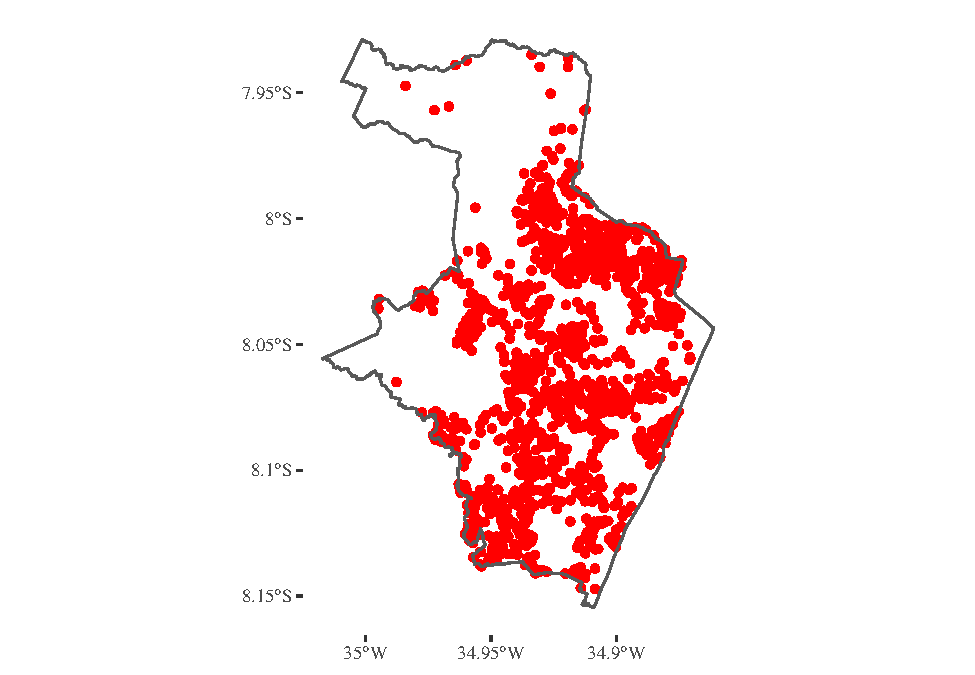
\includegraphics{Moral_Communities_and_Crime_v1_files/figure-latex/plot-crime-1} \hfill{}

\caption{\label{fig:plot-crime}Lethal and Intentional Violent Crime in Recife}\label{fig:plot-crime}
\end{figure}

In addition to places of worship, the National Register of Addresses for
Statistical Purposes was queried to extract facilities other than places
of worship. As discussed above, the idea is to identify points of
reference that can be used as controls, having a neutral morality
profile. For the sake of the present study, we selected pharmacies, ice
cream shops, and bakeries to construct our control group. These three
types of establishments comply with the criteria of being morally
neutral and having a spatial distribution commensurate with places of
worship. Figure 2 shows the spatial distribution of the control
establishments, namely pharmacies, bakeries, and ice cream shops in the
city of Recife. Note the similarity between the maps. As expected, there
are differences in the number of points, but the locations of cases and
controls are quite similar.

\begin{figure}

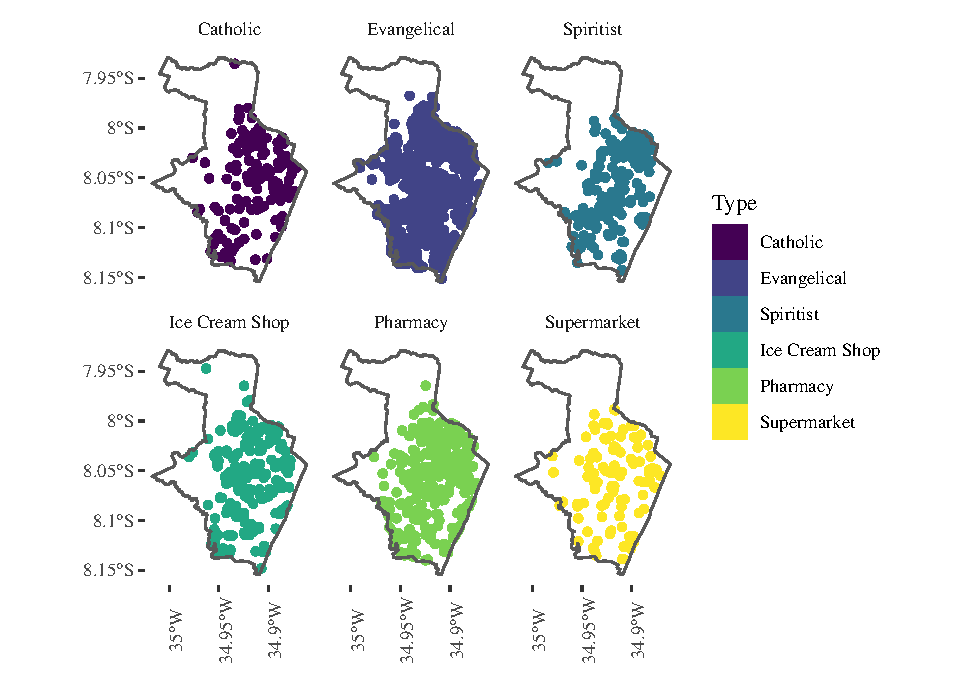
\includegraphics{Moral_Communities_and_Crime_v1_files/figure-latex/plot-events-1} \hfill{}

\caption{\label{fig:plot-events}Places of Worship and Commercial Establishments in Recife}\label{fig:plot-events}
\end{figure}

\begin{figure}

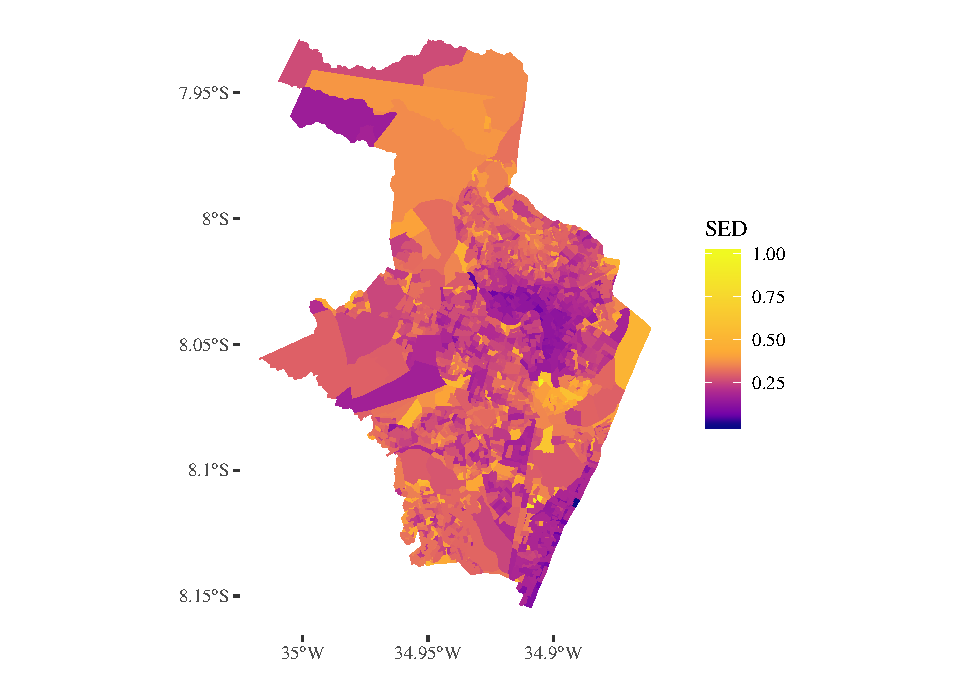
\includegraphics{Moral_Communities_and_Crime_v1_files/figure-latex/plot-sed-1} \hfill{}

\caption{\label{fig:plot-sed}Socio-Economic Deprivation in Recife}\label{fig:plot-sed}
\end{figure}

\hypertarget{results}{%
\section{Analysis and results}\label{results}}

\hypertarget{quadrat-analysis-1}{%
\subsection{Quadrat Analysis}\label{quadrat-analysis-1}}

\begin{figure}
\centering
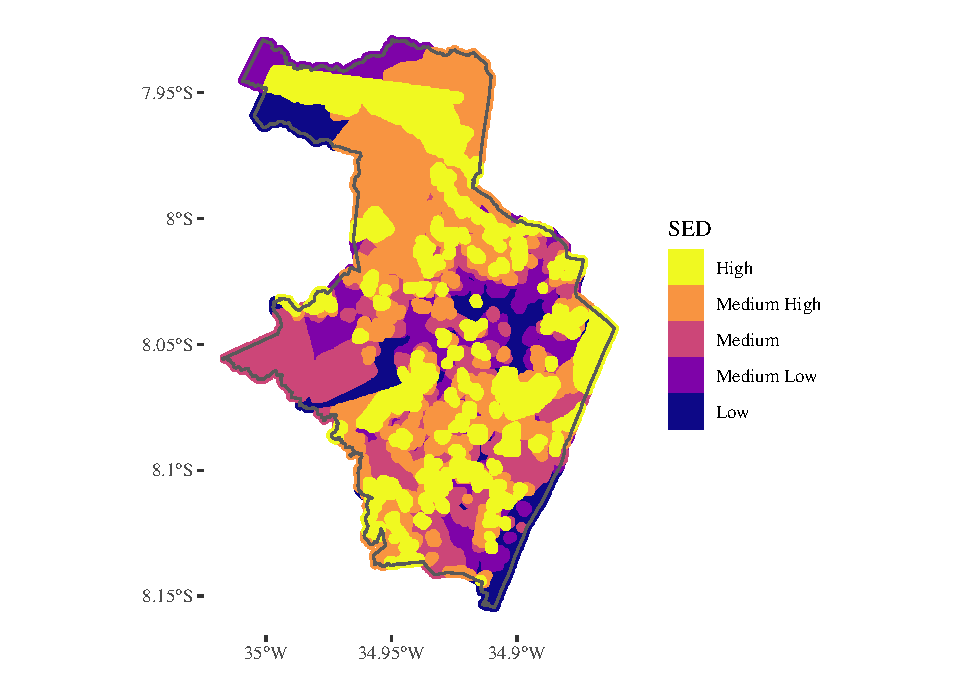
\includegraphics{Moral_Communities_and_Crime_v1_files/figure-latex/plot-sed-as-quintiles-1.pdf}
\caption{\label{fig:plot-sed-as-quintiles}Socio-Economic Deprivation as
Quintiles}
\end{figure}

Calculate the intensity of other ppp by quadrat:

\begin{figure}
\centering
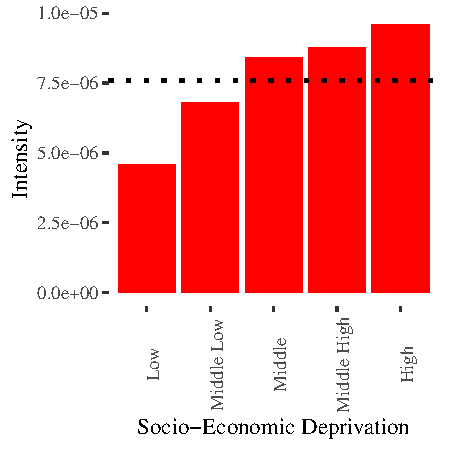
\includegraphics{Moral_Communities_and_Crime_v1_files/figure-latex/plot-crime-quadrat-1.pdf}
\caption{\label{fig:plot-crime-quadrat}Intensity of crime by level of
Socio-Economic Deprivation; the dotted line indicates the global
intensity of crime}
\end{figure}

\begin{figure}
\centering
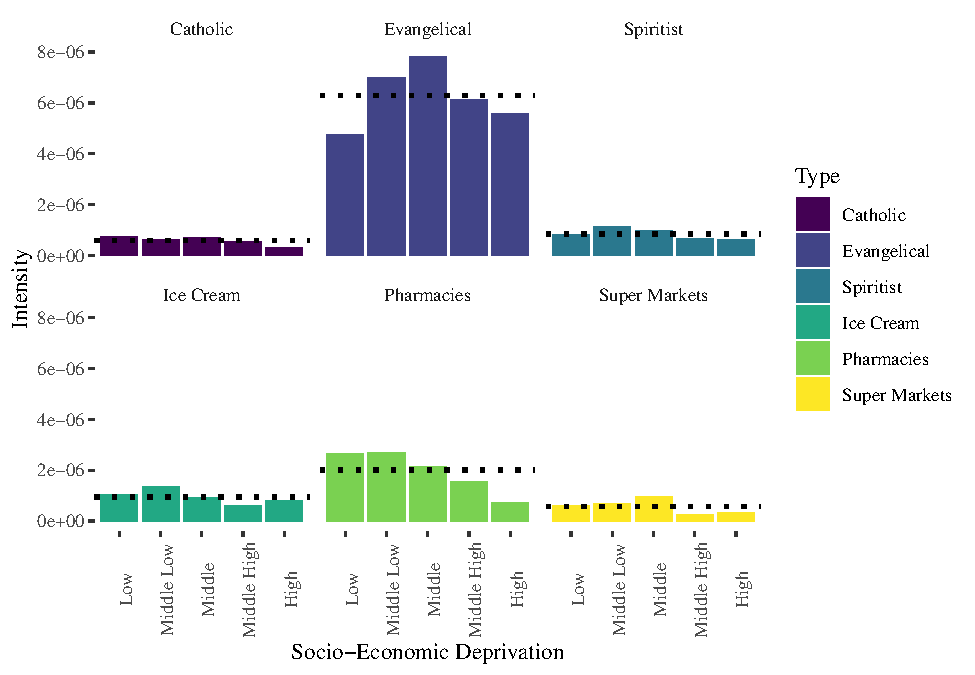
\includegraphics{Moral_Communities_and_Crime_v1_files/figure-latex/plot-events-quadrat-1.pdf}
\caption{\label{fig:plot-events-quadrat}Intensity of places of worship
and commercial establishments by level of Socio-Economic Deprivation;
the dotted lines indicates the respective global intensities}
\end{figure}

\hypertarget{relative-intensity-1}{%
\subsection{Relative Intensity}\label{relative-intensity-1}}

\hypertarget{conclusions}{%
\section{Conclusions}\label{conclusions}}

Words go here.

\hypertarget{references}{%
\section*{References}\label{references}}
\addcontentsline{toc}{section}{References}

\hypertarget{refs}{}
\leavevmode\hypertarget{ref-Abdullah2018amenities}{}%
Abdullah, Snhs, F. A. Bohani, Z. A. Nazri, Y. Jeffry, M. A. Abdullah, M.
N. Junoh, and Z. A. Kasim. 2018. ``Amenities Surrounding Commercial
Serial Crime Prediction at Greater Valley and Kuala Lumpur Using K-Means
Clustering.'' Journal Article. \emph{Jurnal Teknologi} 80 (4): 43--53.
\href{\%3CGo\%20to\%20ISI\%3E://WOS:000437011000005}{\textless{}Go to ISI\textgreater{}://WOS:000437011000005}.

\leavevmode\hypertarget{ref-Becker2017analise}{}%
Becker, Kalinca Léia, and Ana Lúcia Kassouf. 2017. ``Uma análise Do
Efeito Dos Gastos Públicos Em Educação Sobre a Criminalidade No
Brasil.'' \emph{Economia E Sociedade} 26 (1): 215--42.

\leavevmode\hypertarget{ref-Brower2007spatial}{}%
Brower, A. M., and L. Carroll. 2007. ``Spatial and Temporal Aspects of
Alcohol-Related Crime in a College Town.'' Journal Article.
\emph{Journal of American College Health} 55 (5): 267--75.
\url{https://doi.org/10.3200/jach.55.5.267-276}.

\leavevmode\hypertarget{ref-Davignon2015christian}{}%
Davignon, P., and R. A. Thomson. 2015. ``Christian Colleges and
Universities as Moral Communities: The Effects of Institutional
Characteristics on Student Religiosity.'' Journal Article. \emph{Review
of Religious Research} 57 (4): 531--54.
\url{https://doi.org/10.1007/s13644-015-0214-5}.

\leavevmode\hypertarget{ref-Deryol2016crime}{}%
Deryol, R., P. Wilcox, M. Logan, and J. Wooldredge. 2016. ``Crime Places
in Context: An Illustration of the Multilevel Nature of Hot Spot
Development.'' Journal Article. \emph{Journal of Quantitative
Criminology} 32 (2): 305--25.
\url{https://doi.org/10.1007/s10940-015-9278-1}.

\leavevmode\hypertarget{ref-Doran2011putting}{}%
Doran, Bruce J, and Melissa B Burgess. 2011. \emph{Putting Fear of Crime
on the Map: Investigating Perceptions of Crime Using Geographic
Information Systems}. Springer Science \& Business Media.

\leavevmode\hypertarget{ref-Foster2010neighbourhood}{}%
Foster, S., B. Giles-Corti, and M. Knuiman. 2010. ``Neighbourhood Design
and Fear of Crime: A Social-Ecological Examination of the Correlates of
Residents' Fear in New Suburban Housing Developments.'' Journal Article.
\emph{Health \& Place} 16 (6): 1156--65.
\url{https://doi.org/10.1016/j.healthplace.2010.07.007}.

\leavevmode\hypertarget{ref-Furr2010metric}{}%
Furr-Holden, C. D. M., K. D. M. Campbell, A. J. Milam, M. J. Smart, N.
A. Ialongo, and P. J. Leaf. 2010. ``Metric Properties of the
Neighborhood Inventory for Environmental Typology (Nifety): An
Environmental Assessment Tool for Measuring Indicators of Violence,
Alcohol, Tobacco, and Other Drug Exposures.'' Journal Article.
\emph{Evaluation Review} 34 (3): 159--84.
\url{https://doi.org/10.1177/0193841x10368493}.

\leavevmode\hypertarget{ref-He2017built}{}%
He, Li, Antonio Páez, and Desheng Liu. 2017. ``Built Environment and
Violent Crime: An Environmental Audit Approach Using Google Street
View.'' Journal Article. \emph{Computers, Environment and Urban Systems}
66: 83--95.
\url{https://doi.org/http://dx.doi.org/10.1016/j.compenvurbsys.2017.08.001}.

\leavevmode\hypertarget{ref-Lipton2008spatial}{}%
Lipton, R., A. Banerjee, D. Levy, N. Manzanilla, and M. Cochrane. 2008.
``The Spatial Distribution of Underage Tobacco Sales in Los Angeles.''
Journal Article. \emph{Substance Use \& Misuse} 43 (11): 1597--1617.
\url{https://doi.org/10.1080/10826080802241110}.

\leavevmode\hypertarget{ref-Loukaitou2001measuring}{}%
Loukaitou-Sideris, A., R. Liggett, H. Iseki, and W. Thurlow. 2001.
``Measuring the Effects of Built Environment on Bus Stop Crime.''
Journal Article. \emph{Environment and Planning B-Planning \& Design} 28
(2): 255--80. \url{https://doi.org/10.1068/b2642r}.

\leavevmode\hypertarget{ref-Menezes2013spatial}{}%
Menezes, T., R. Silveira-Neto, C. Monteiro, and J. L. Ratton. 2013.
``Spatial Correlation Between Homicide Rates and Inequality: Evidence
from Urban Neighborhoods.'' Journal Article. \emph{Economics Letters}
120 (1): 97--99. \url{https://doi.org/10.1016/j.econlet.2013.03.040}.

\leavevmode\hypertarget{ref-Murray2013crime}{}%
Murray, J., D. R. D. Cerqueira, and T. Kahn. 2013. ``Crime and Violence
in Brazil: Systematic Review of Time Trends, Prevalence Rates and Risk
Factors.'' Journal Article. \emph{Aggression and Violent Behavior} 18
(5): 471--83. \url{https://doi.org/10.1016/j.avb.2013.07.003}.

\leavevmode\hypertarget{ref-Quick2017influence}{}%
Quick, M., J. Law, and H. Luan. 2017. ``The Influence of on-Premise and
Off-Premise Alcohol Outlets on Reported Violent Crime in the Region of
Waterloo, Ontario: Applying Bayesian Spatial Modeling to Inform Land Use
Planning and Policy.'' Journal Article. \emph{Applied Spatial Analysis
and Policy} 10 (3): 435--54.
\url{https://doi.org/10.1007/s12061-016-9191-5}.

\leavevmode\hypertarget{ref-Traunmuller2011moral}{}%
Traunmuller, R. 2011. ``Moral Communities? Religion as a Source of
Social Trust in a Multilevel Analysis of 97 German Regions.'' Journal
Article. \emph{European Sociological Review} 27 (3): 346--63.
\url{https://doi.org/10.1093/esr/jcq011}.

\leavevmode\hypertarget{ref-Unodc2019executive}{}%
United Nations Office on Drugs and Crime. 2019a. ``Global Study on
Homicide 2019: Executive Summary.'' UNODC Vienna.

\leavevmode\hypertarget{ref-Unodc2019development}{}%
---------. 2019b. ``Global Study on Homicide 2019: Homicide, Development
and the Sustainable Development Goals.'' UNODC Vienna.

\leavevmode\hypertarget{ref-Warner2019neighborhood}{}%
Warner, B. D., and R. H. Konkel. n.d. ``Neighborhood Churches and Their
Relationship to Neighborhood Processes Important for Crime Prevention.''
Journal Article. \emph{Journal of Urban Affairs}.
\url{https://doi.org/10.1080/07352166.2019.1581030}.

\bibliographystyle{spbasic}
\bibliography{bibliography.bib}

\end{document}
